\section{(i) Andorra Data Observatory}\label{sec:andorra-data-observatory}
{
    As part of the collaboration with the Andorran government, a set of tools to analyze, visualize, and extract insights on large public events were create. This section details a data-visualization platform that (i) models the trajectories of large amount of individuals and visitors in several public gathering in Andorra's major cities, (ii) use Agent Based modeling (ABM) to analyze these patterns, and (iii) extract relevant insights and conclusions from these insights.

    \begin{figure}[h]
        \begin{center}
            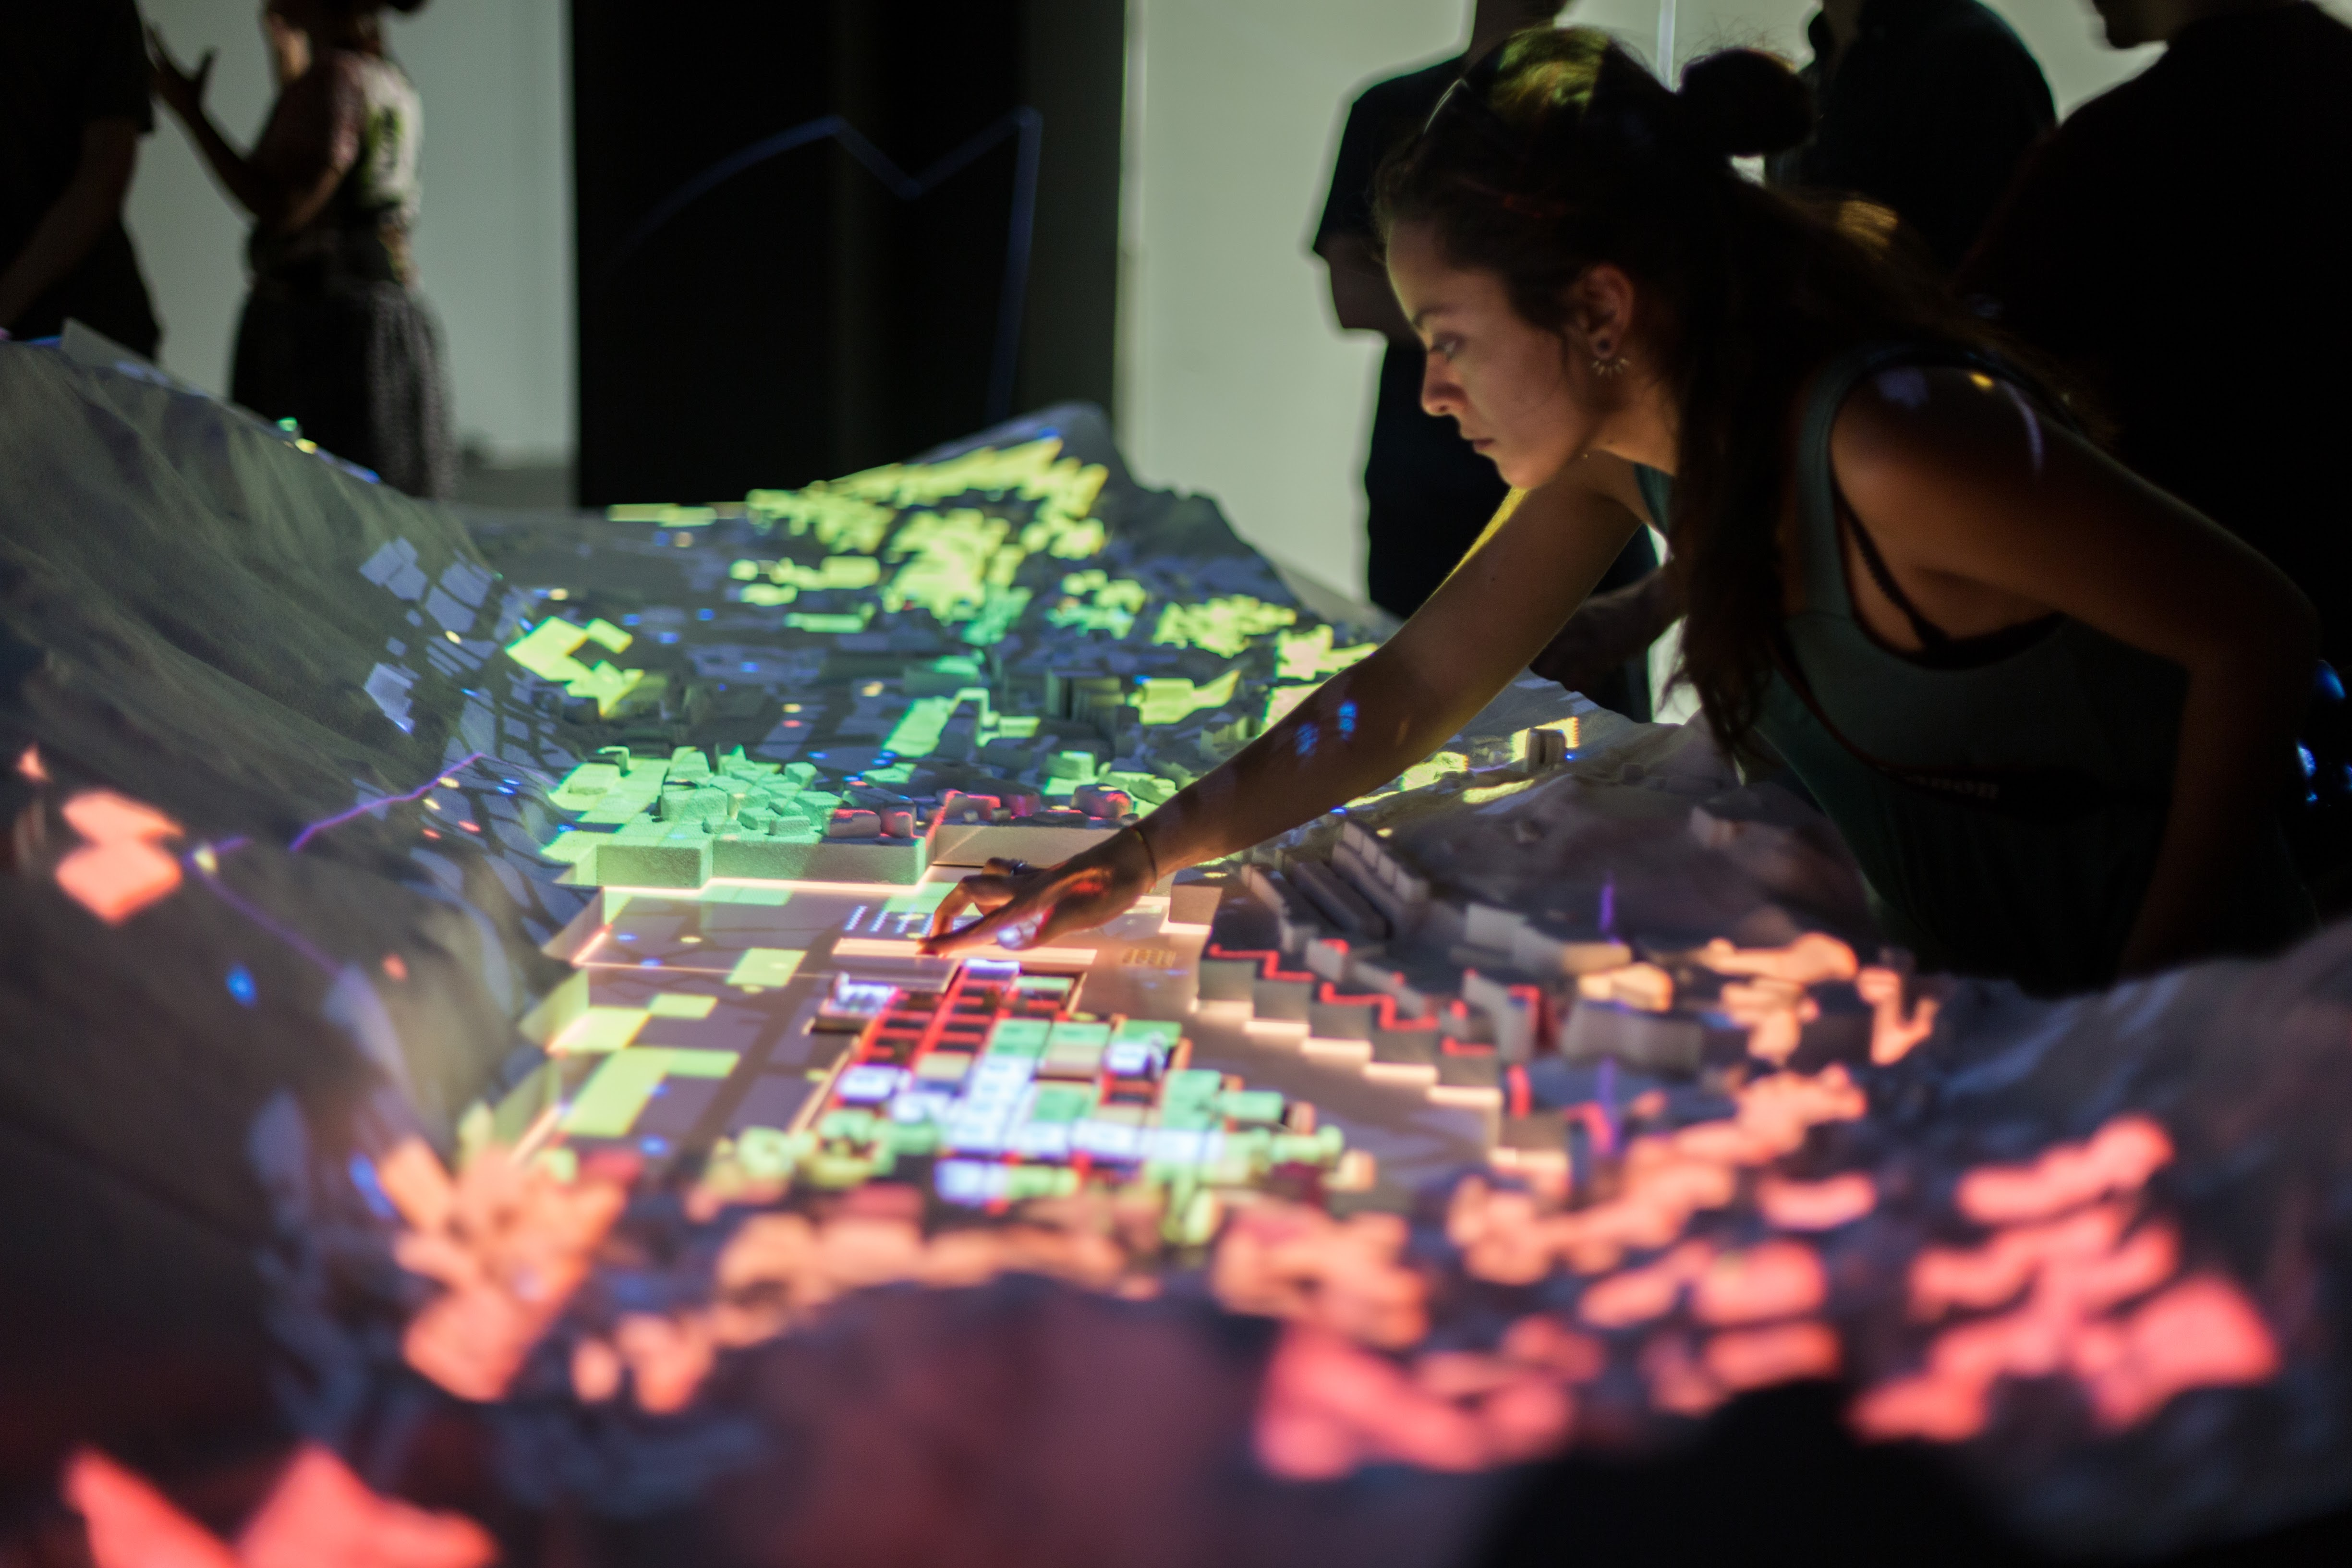
\includegraphics[width=1\textwidth]{chapters/insight/and_abm/figures/and_cityscope.jpg}
        \end{center}
        \caption{CityScope Andorra at the City Science Lab in Caldea, Andorra la Vella. Built in 2016, this platform was one of the first to serve as an interactive, real-time tool for urban decision making. Here, a user interacts with a Tangible User Interface to asses the impacts of different interventions in the city center.}
        \label{fig:and_cityscope}
    \end{figure}

    \subsection{Events}
    {
        Andorra has a population of nearly eighty thousand, and hosts more than eight million visitors in a normal year, many of them as tourists\footnote{According to the \textit{Departament d\'Estad\'istica}, Andorra had approximately eight million visitors in 2016: 4.2M Spanish, 3.2M French, and 0.6M from other nationalities.}. The tourism sector accounts for $\sim$80\% of Andorra's GDP and thus large public events are critical for the local economy \cite{CIA}. This work focuses on observing the mobility patterns of both pedestrians and vehicles, as a product of tourists and visitors' attendance at annual events in Andorra. The work focuses on the following events: (i) \textit{Cirque du Soleil: VISION} and (ii) \textit{Le Tour de France}, both took place in 2016.
        \newline
        `Scalada' by \textit{Cirque du Soleil: VISION}, is a series of indoor, summertime shows, taking place between Tuesdays to Saturdays, July 2\textsuperscript{nd} - July 30\textsuperscript{th}, 2016. VISION's venue has a capacity for 5000 people per performance. \textit{Le Tour de France} is an annual multiple stage bicycle race held in France, which occasionally passes through nearby EU countries. In 2016, Andorra hosted \textit{Le Tour de France} Stage 9 in its mountain area (Arcal\'is, Ordino) as well as the departure of Stage 10 in the city center (Escaldes, Escaldes-Engordany).
    }

    \subsection{Data and Method}
    {
        Call Detail Records (CDR) are digital records gathered by the mobile network operator used for billing purposes. Observations are triggered by mobile phones actions such as phone calls, text messages, and cellular data. This source of data is broadly used in the research community, since it contains spatial information, allowing to conduct flow analyses \cite{Blondel2015, ccolak2015analyzing, Ratti2006}. As part of this work, Andorra Telecom shared nearly three years of CDR data (2014-2016)\footnote{In order to comply with privacy policies, all personal identifiers, such as names and mobile phone numbers, were anonymized based on a Secure Hash Algorithm (SHA-512), a one-direction encryption method preventing the retrieval of the information obscured.}. Each entry in the CDR contains unique anonymized caller id, the date and time of the call, call duration, and the id of the Base Transceiver Station tower, as shown in table \eqref{f:CDRSample}. with this data, tower-to-tower origin and destination matrices (OD) for each individual were computed.


        \begin{table}
            \begin{center}
                \begin{tabular}{c|cccc}
                    \hline
                    Anonymized ID & Call Date & Call Time & Duration & towerID \\
                    \hline
                    iAAJKnPAa5    & 20160716  & 09:34:13  & 18       & 2       \\
                    iAAJKnPAa5    & 20160716  & 10:21:43  & 156      & 6       \\
                    iAAJKnPAa5    & 20160716  & 13:02:37  & 38       & 10      \\
                    \hline
                \end{tabular}
                \caption{Sample of a CDR observation}
                \label{f:CDRSample}
            \end{center}
        \end{table}


        \subsubsection{Road Network}
        {
            CDR data provide scarce localizing per given user. The nature of these data dictates simplified tower-to-tower OD matrices that correspond to linear, non geographically accurate vectors. In order to correlate these trajectories to the existing road network, users are constrained to roam along a graph topology \cite{Gonzalez2008}. Roads of different types are set to bound different mobility modes (primary, secondary, residential, or pedestrian). In order to compute a more accurate shortest path, the road network is considered as a weight-directed graph used to constrain the behavior of users. The edge direction represents the directionality of the road; The weight combines the speed limit of the road and the number of user present on that road.
        }

        \subsubsection{POIs and Amenities}
        {
            Given the degree of noise in CDR data, urban amenities, such as restaurants, hotels, and other Points Of Interest, were used to anchor destination points of users. The geolocation of amenities was gathered using several public APIs, such as TripAdvisor and Yelp, as well as the \textit{Andorra Turisme} office.
        }
    }

    \subsection{System Design}
    {
        Processing the LBS dataset, and constraining the agents' movement to the road network and POIs, was done using GAMA, an Agent Based modeling (ABM) software \cite{grignard2013gama} and Processing \cite{reas2007processing}. Using a Tangible User Interface (TUI), users could interact with the simulations, and trigger different visualization layers. The three main classes in the model are an abstraction of the (i) environment (cell towers, roads, and amenities), (ii) mobile agents (people and vehicles), and (iii) interactive grid. The rest of this section details the implementation of the ABM and the visualization of the results on a TUI.

        \begin{figure}[h]
            \begin{center}
                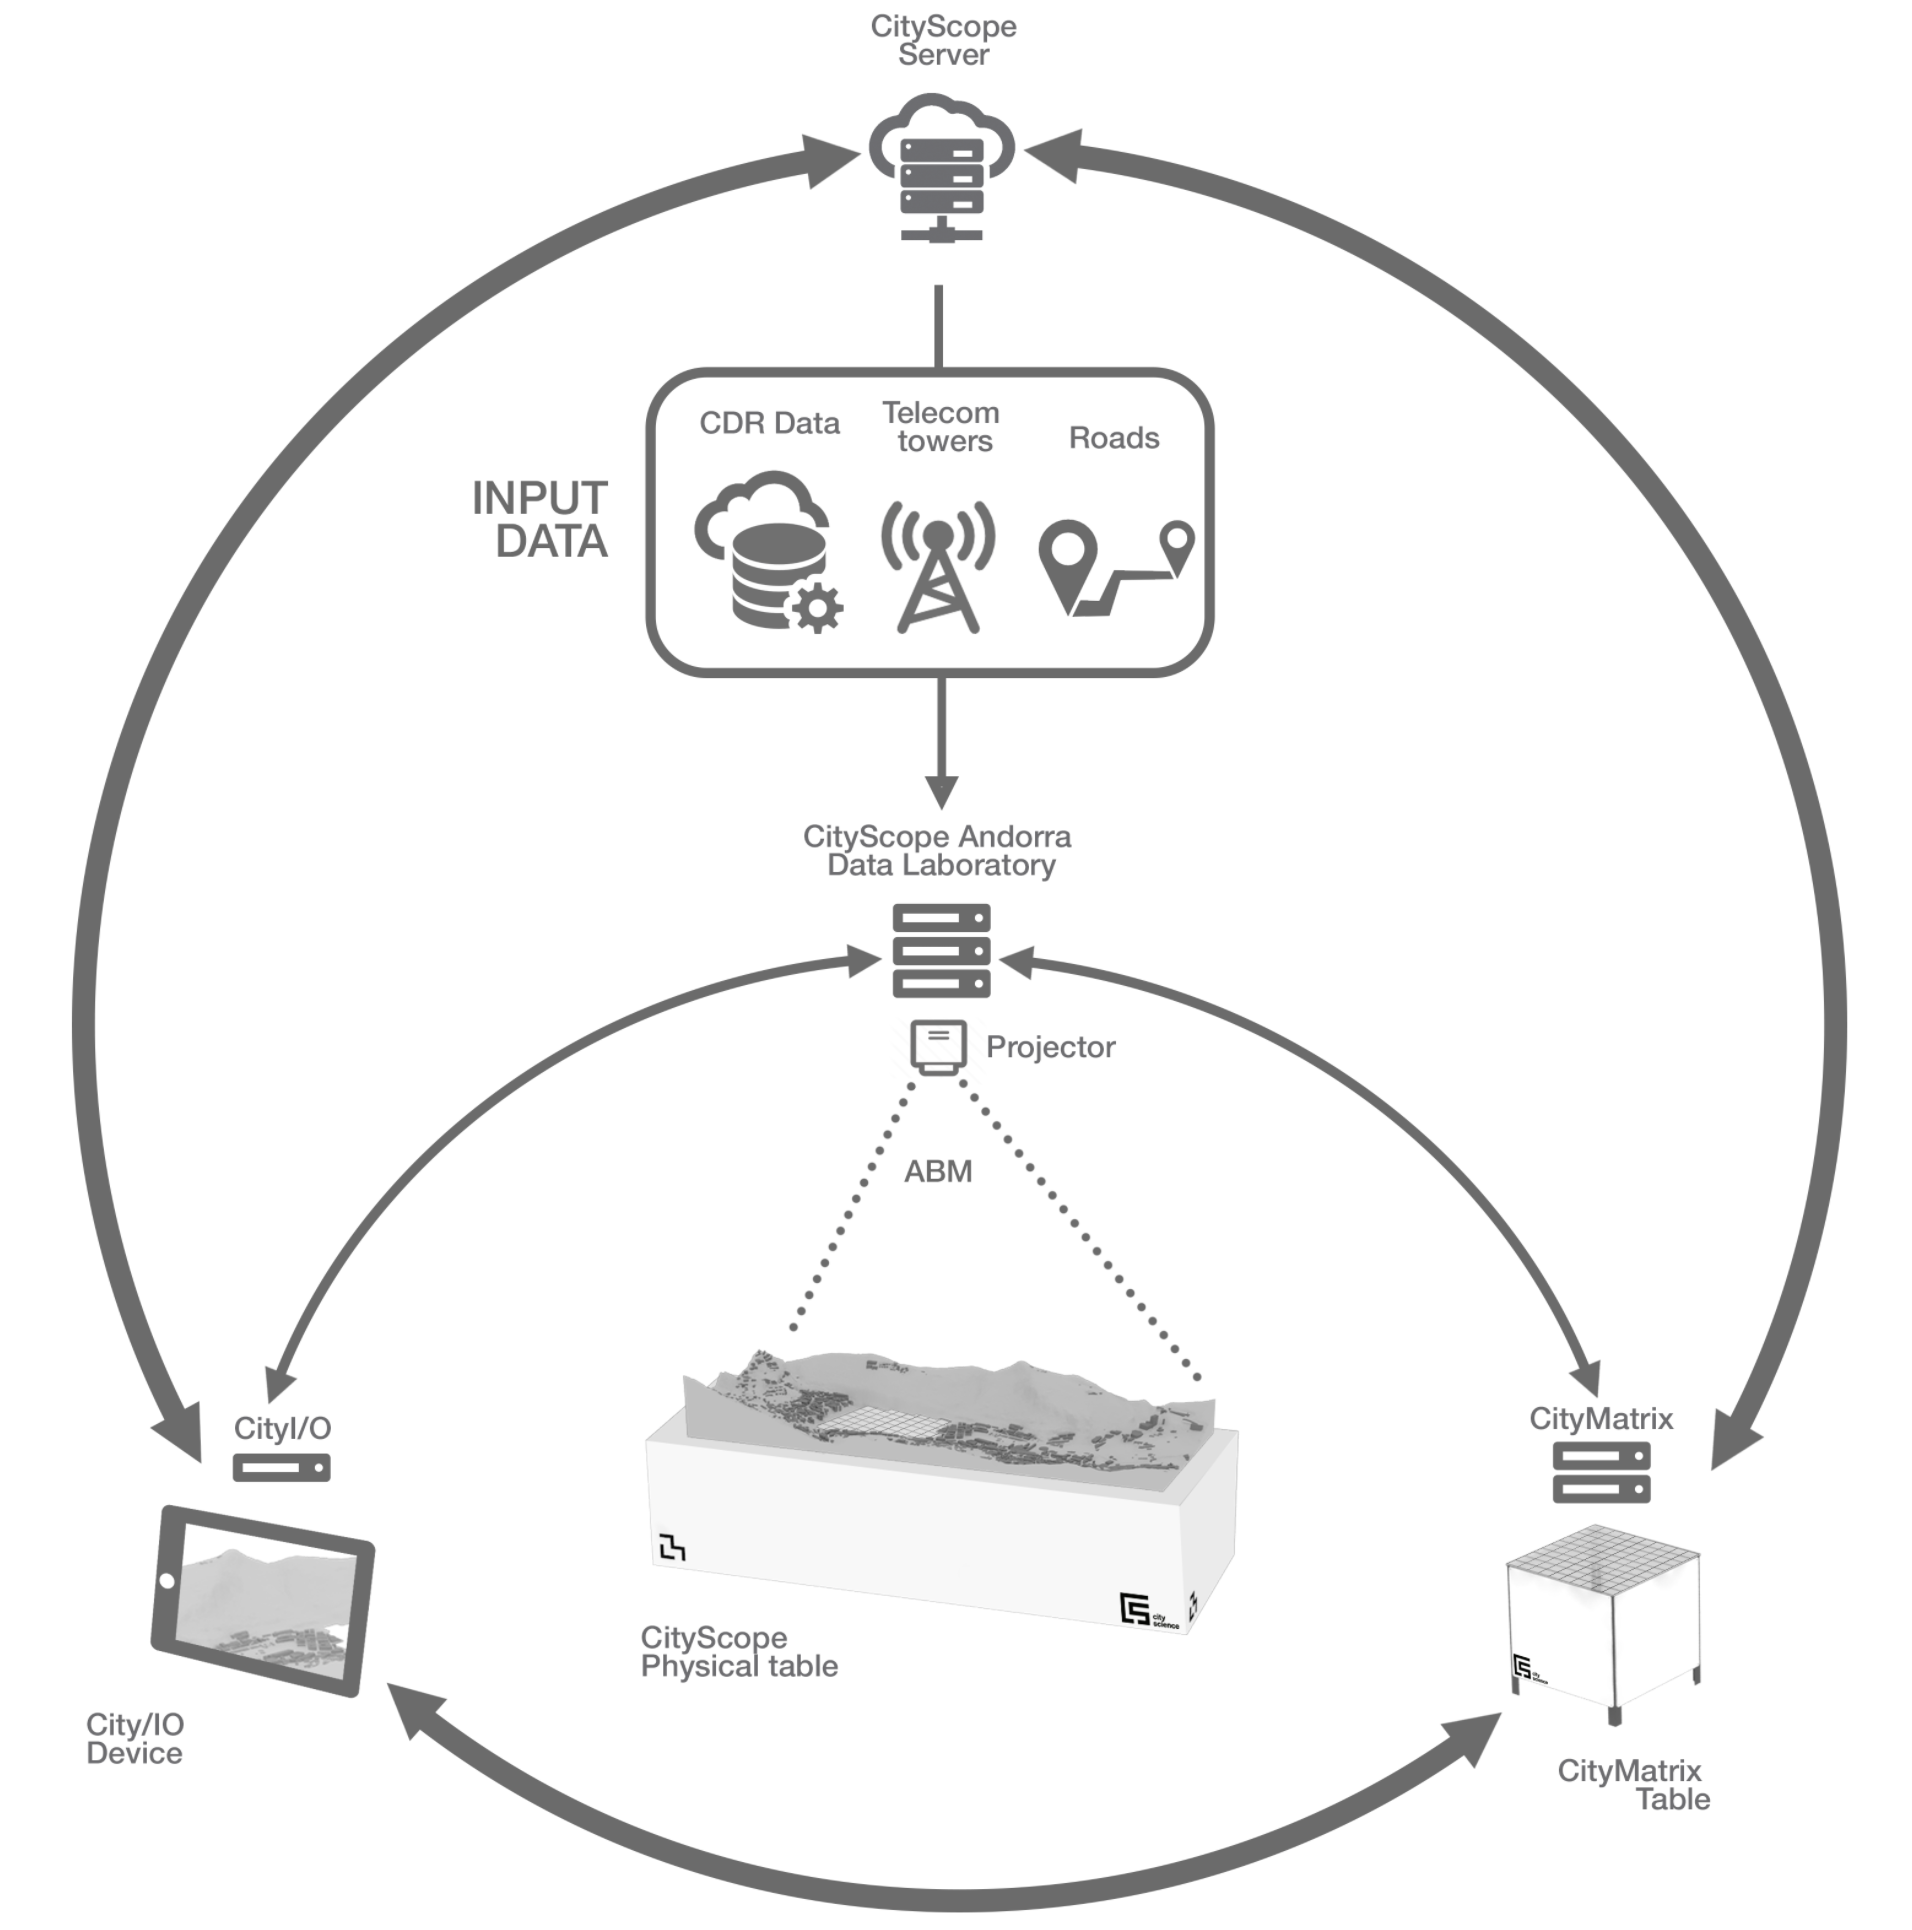
\includegraphics[width=0.4\textwidth]{chapters/insight/and_abm/figures/and_cdr_arch.png}
            \end{center}
            \caption{CityScope Andorra data pipelines and TUI. The ABM is computed from both static (GIS) and dynamic (telecom) datasets. It reacts to changes occurring on auxiliary interfaces (CityScopeAR, CityMatrix) and recompute the simulation in accordance.}
            \label{fig:and_cdr_arch}
        \end{figure}


        \subsubsection{Agent Based Model}
        {
            The ABM uses several datasets to characterize agents' behavior in the city: (i) telecom data, (ii) road network, and (iii) amenities and POIs data.
            \newline
            \textbf{Agents:} The virtual environment (`world') is populated with independent agents, each with an assigned set of variables that influence their behavior whenever changes occurs, either locally or at the surrounding environment. \textbf{State:} The agent's variables are (1) agent's country of residence; (2) origin location: defined using telecom data; (3) preferred destination, generated by predefined or dynamically added urban anchors; (4) distance traveled; (5) speed of movement; and (6) passable network nodes. \textbf{Behavior:} The agent's trajectory is determined by the OD matrix computed from the CDR data. The path is computed by constraining the OD to the local road network. The agent's destination is anchored to the amenity closest to the cell tower coverage where its action was recorded when terminated. The chosen amenity depends on the agent's country of residence and the language affinity of the amenities. Depending on its speed (time difference between origin and destination location), the agent will be considered as a pedestrian (solid circle) or as a vehicle (stroke circle).
            \newline
            Agents can adapt themselves to several dynamic factors: (i) traffic congestion: in case of severe congestion, a pathfinding method is called to recalculate an alternative route. If a road is busy, the agent will recompute a shortest path to its destination in order to avoid that road; and (ii) amenity occupancy: if the amenity assigned as destination is flagged as full, the agent can select another amenity close-by to its prior destination. Once agents reach their destination, they stay there for a few iterations. The number of iterations is defined by the average time spent on those places, retrieved from the different APIs.
        }

        \subsubsection{Visualization}
        {
            The ABM was displayed via three main visual layers: (i) Spatial elements, such as geography, buildings, amenities, cell towers, and roads, (ii) Pedestrian and vehicular movement from the ABM, and (iii) Amenities' popularity and density. Pedestrians were represented by solid circles and vehicles by stroke circles, colored according to their origin country: Orange refers to visitors from Spain, blue for France, and white for other countries\footnote{This classes were suggested by \textit{Departament d'Estad\'itica d'Andorra}, although the telecom data has more detailed classification via the IMSI property}.
            The visual representation of POIs and amenities echos the number of agents currently resting at a given location, indicating the activity level in a place. The large white circle highlights the location where the show was taking place. The simulation concluded that 5,174 visitors attendees at the same time, within a reasonable range of \textit{Andorra Turisme} official tally of 4,540 visitors.
            \newline
            Unlike \textit{Cirque du Soleil}, \textit{Le Tour de France} is an outdoor event in which no ticketing process can help assess attendance. Therefore, an aggregated heatmap representation was used to summarize global activity, and provide geo-located attendance estimates. Figure \eqref{fig:and_cdr_viz} show occupancy levels for \textit{Le Tour de France} during July 12\textsuperscript{th}. The race starting point was at Escaldes-Engordany, shown as the most active area in Figure \eqref{fig:and_cdr_viz}, with large concentration on the left side.

            \begin{figure}[h]
                \begin{center}
                    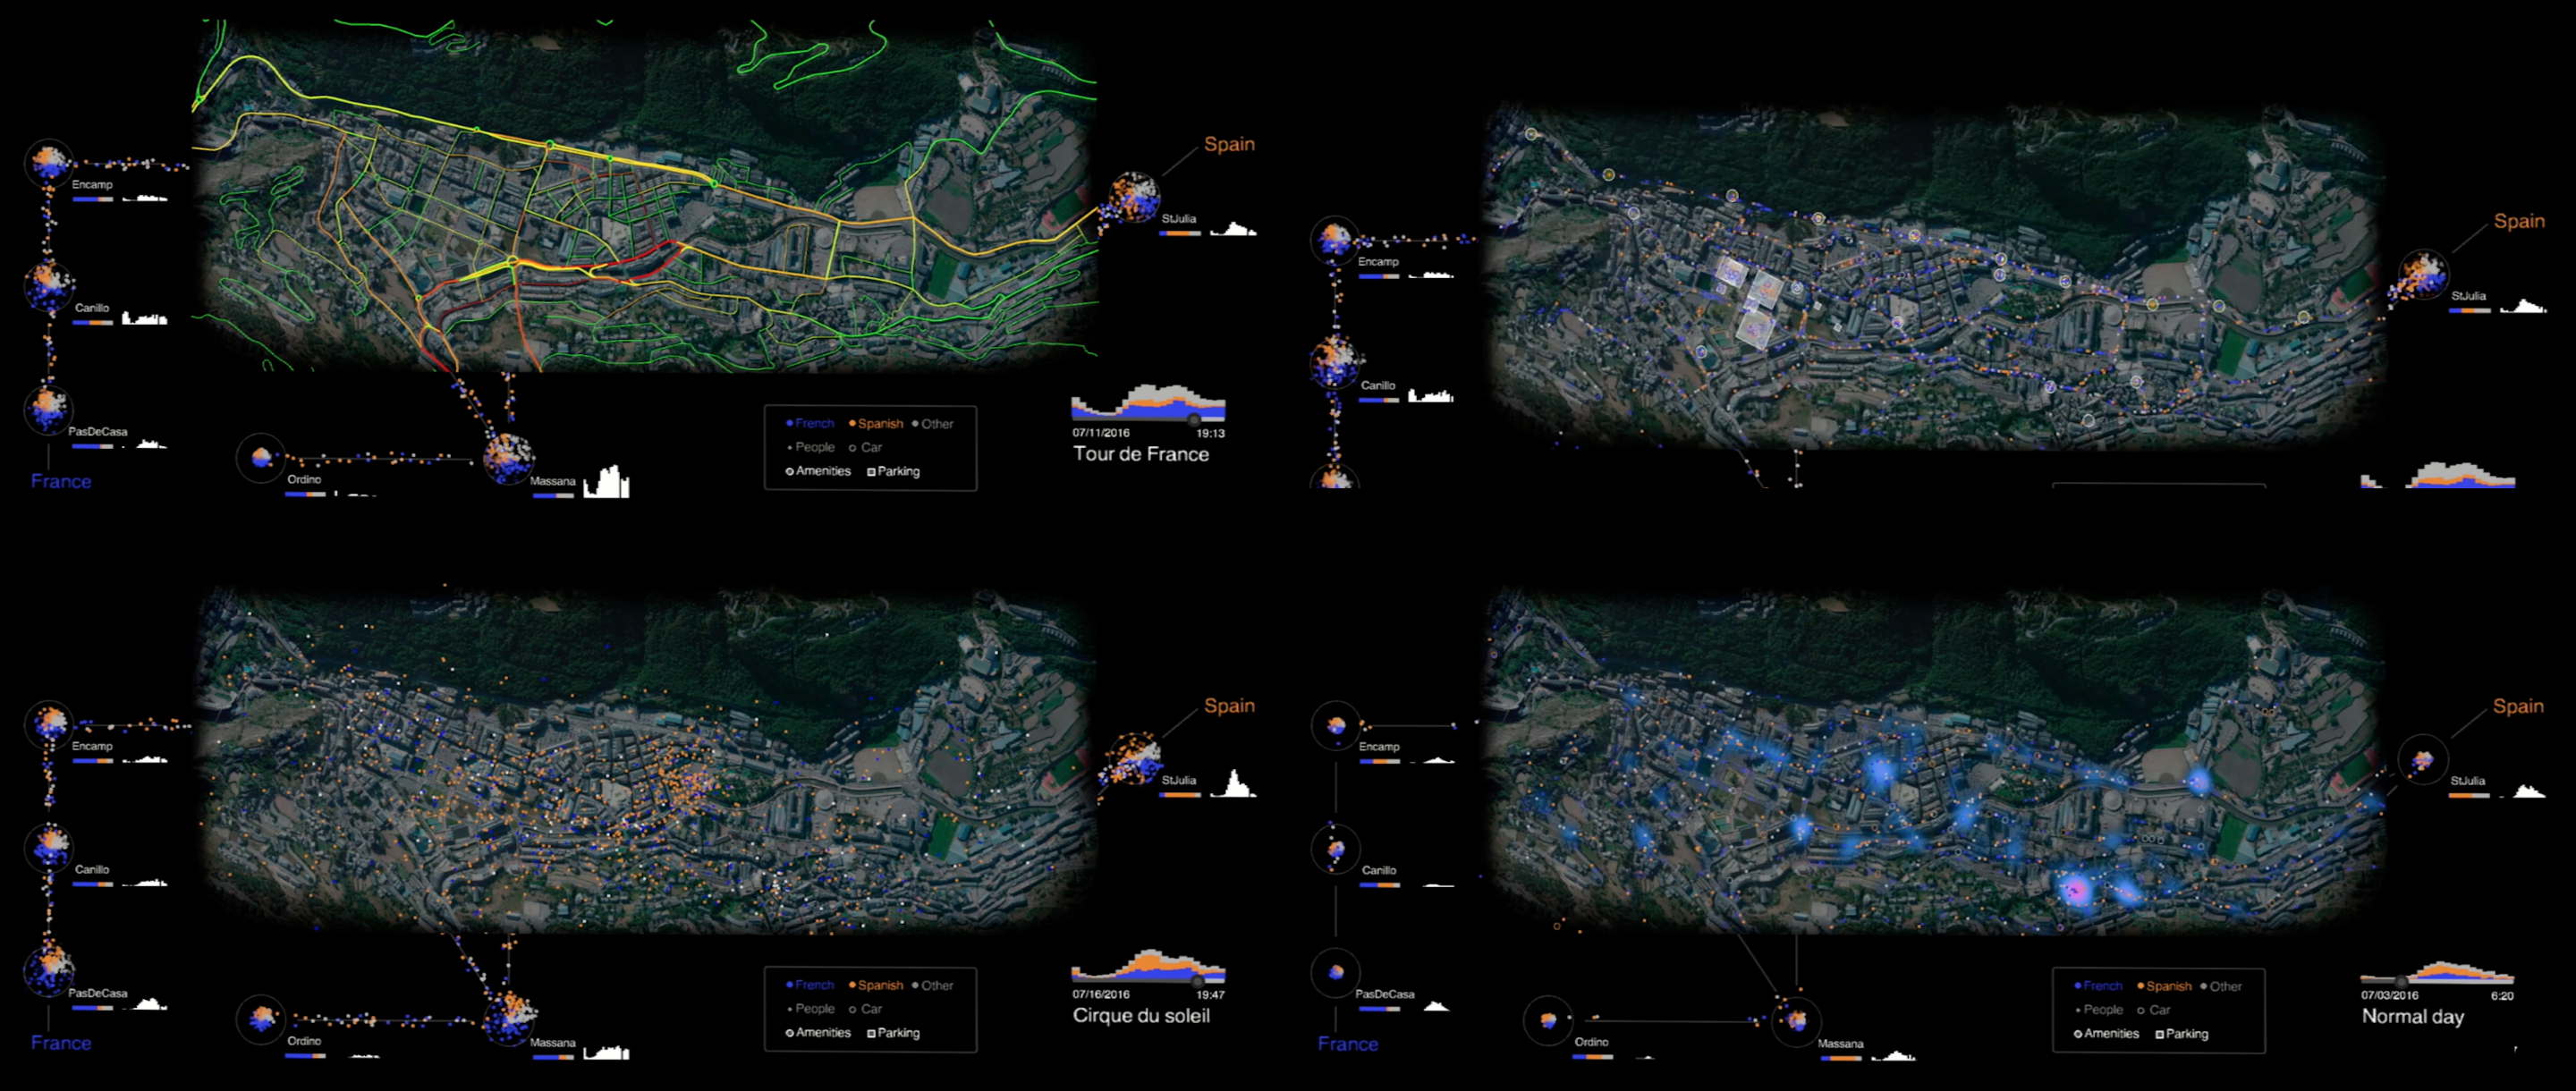
\includegraphics[width=1\textwidth]{chapters/insight/and_abm/figures/and_cdr_viz.png}
                \end{center}
                \caption{
                    (top left) Aggregated congestion for the entire day during \textit{Le Tour de France}. (top right) Travel patterns anchored to the road network and associated to inferred amentias as destination points. (bottom left) Raw CDR data; points represent locations recorded from cell towers. (bottom right) `Hot-spots' agglomerated in areas where multiple simulated agents are passing through a given street.
                }
                \label{fig:and_cdr_viz}
            \end{figure}
        }

        \subsubsection{Tangible Layer}
        {
            \begin{figure}[h]
                \begin{center}
                    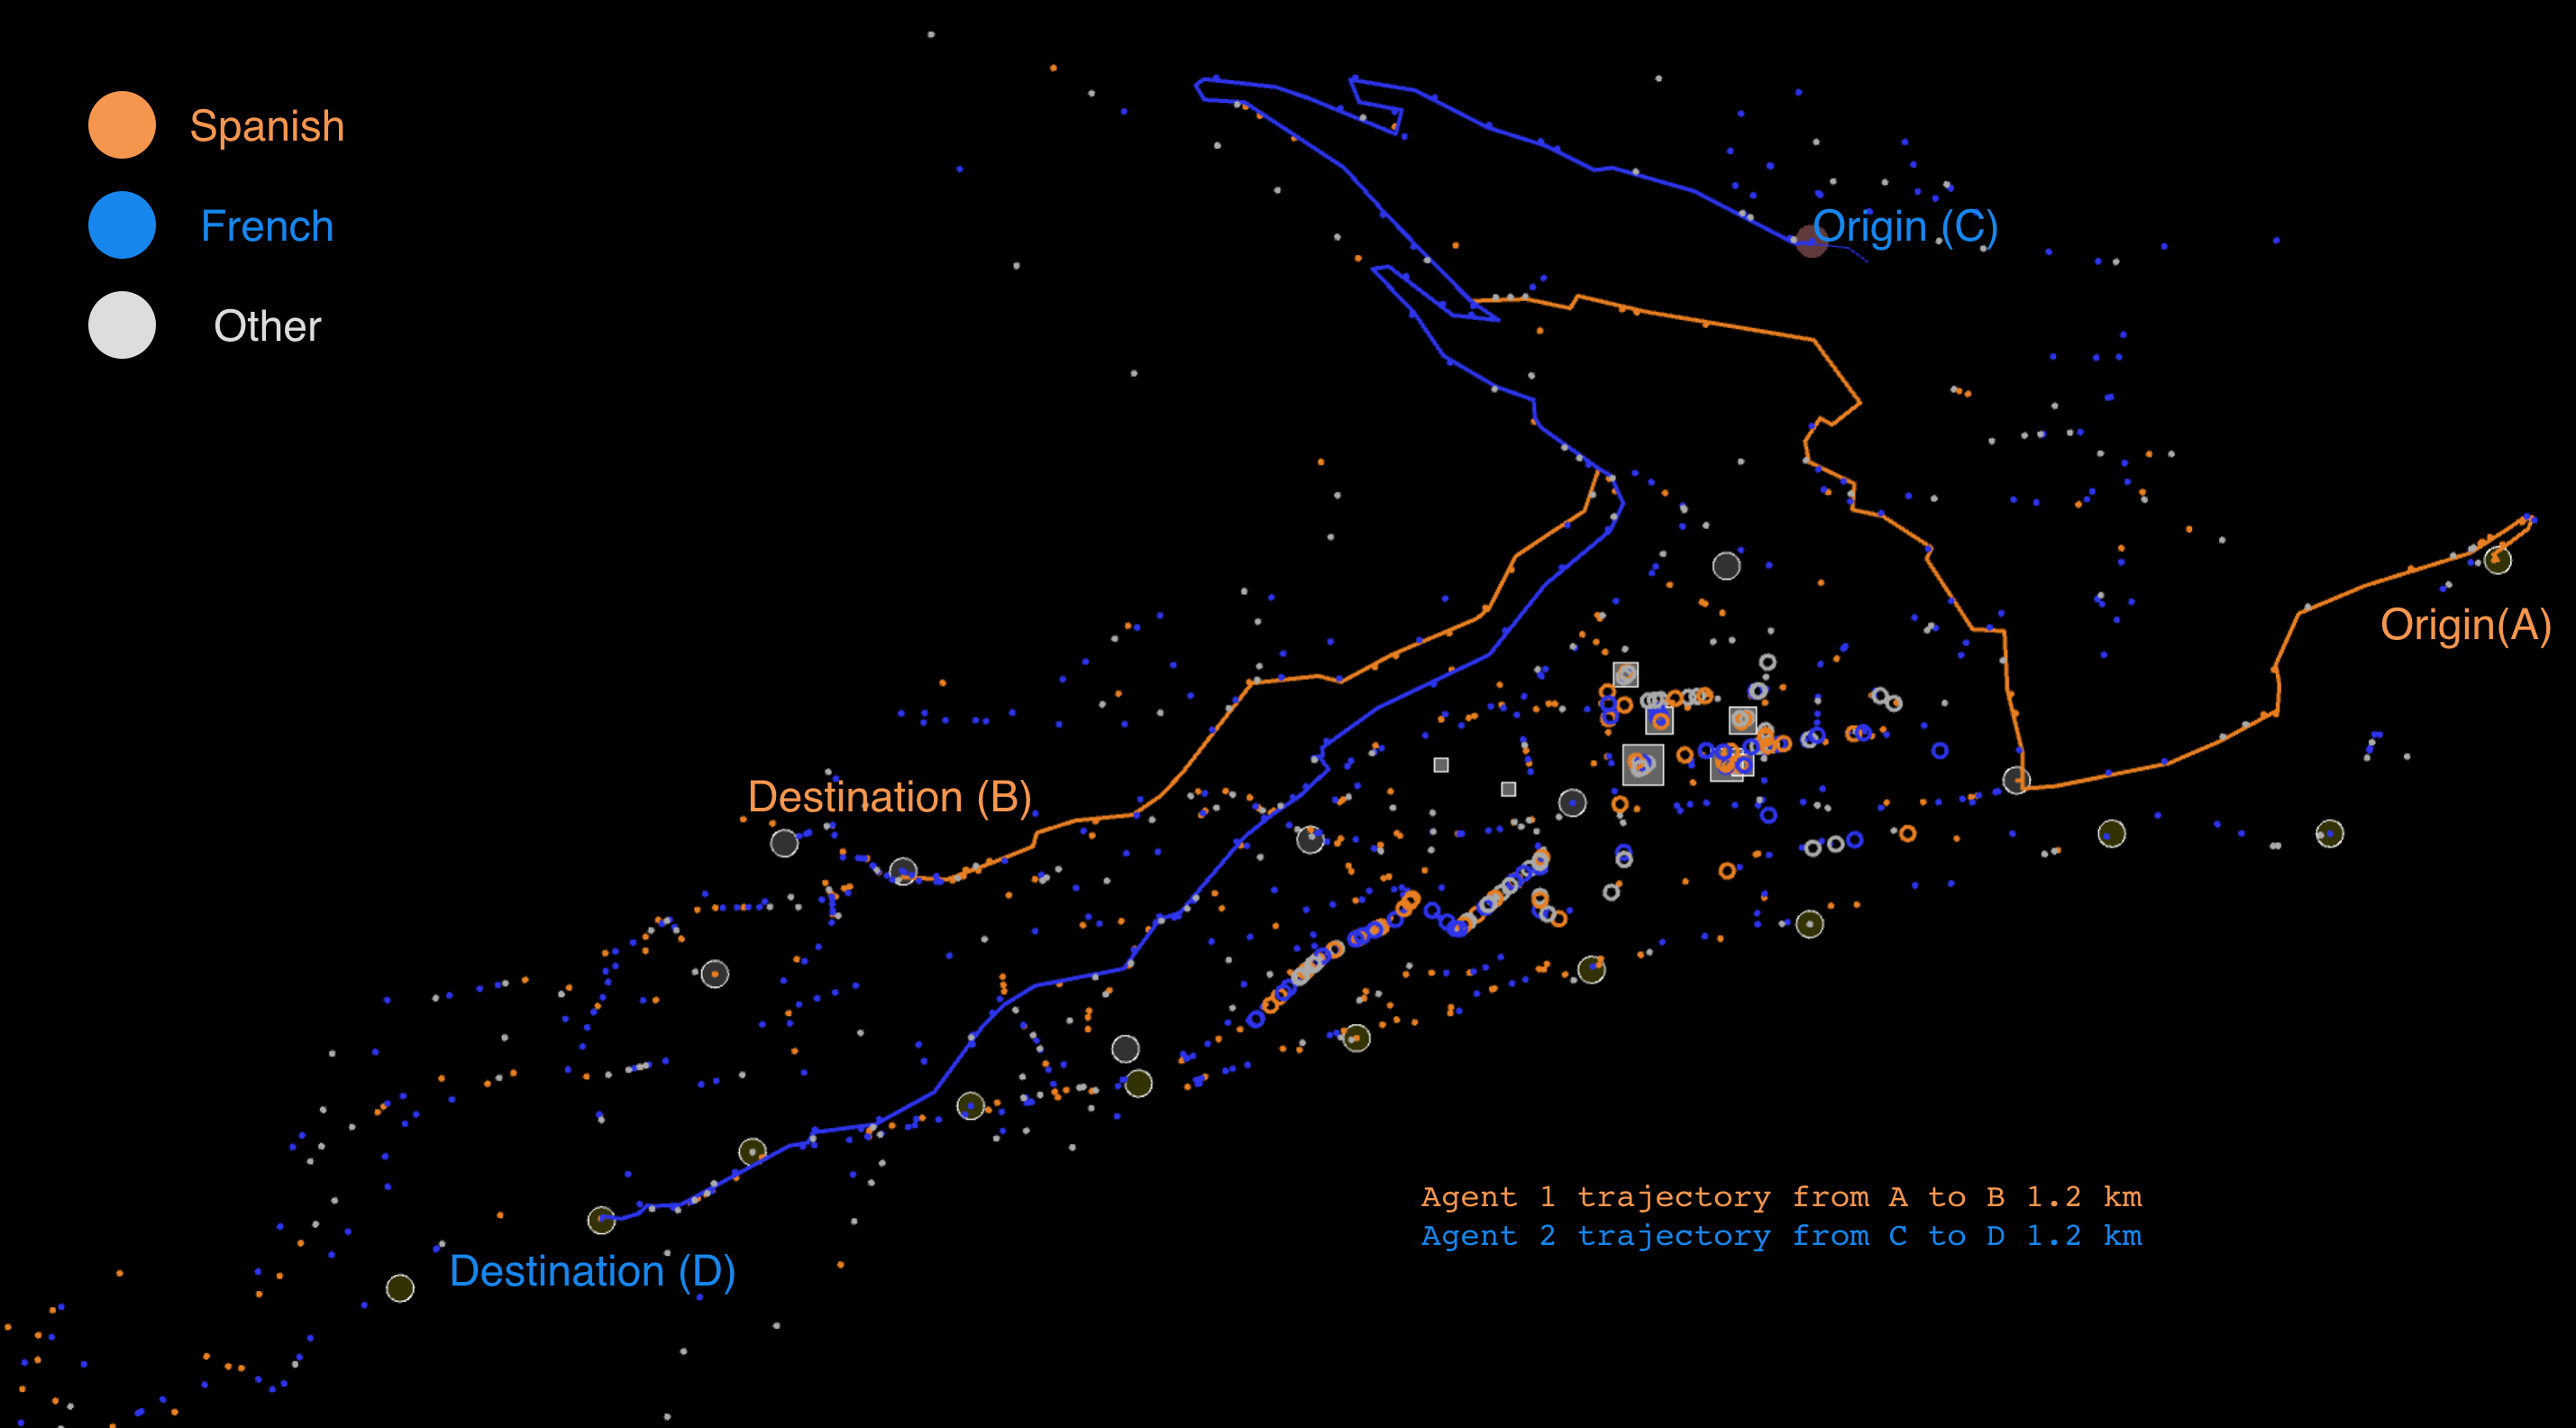
\includegraphics[width=1\textwidth]{chapters/insight/and_abm/figures/trajectory.png}
                \end{center}
                \caption{Trajectories are computed by traversing between the CDR records, and aligning the trip to existing road network. The speed between these points is assumed to be a proxy for mode of transit (faster=car/transit, slower=bikes/foot).}
                \label{fig:and_trajectories}
            \end{figure}

            The Andorra CityScope TUI has three components: (i) A physical 3D model of the city made out of LEGO, (ii) An abstract representation of a redevelopment area at the city's center, and (iii) Augmented Reality (AR) data-visualization system.
            \newline
            In 2016, a physical model was built, consisting of a 3D topographical model of the two main cities in Andorra: Andorra la-Vella and Escaldes-Engordany. The outskirts of these two cities, as well as cities located near the border (Sant Julia de L'oria near the Spanish border and Pas de la Casa near the French border) and the parishes of Canillo, Encamp, Ordino, and La Massana, are abstractly represented using pie-chart like population clusters. A temporal indication of the visitor's flow is displayed using a slider, and the population volume is displayed by a histogram.
        }

        \subsubsection{Augmented Reality}
        {
            \begin{figure}[h]
                \begin{center}
                    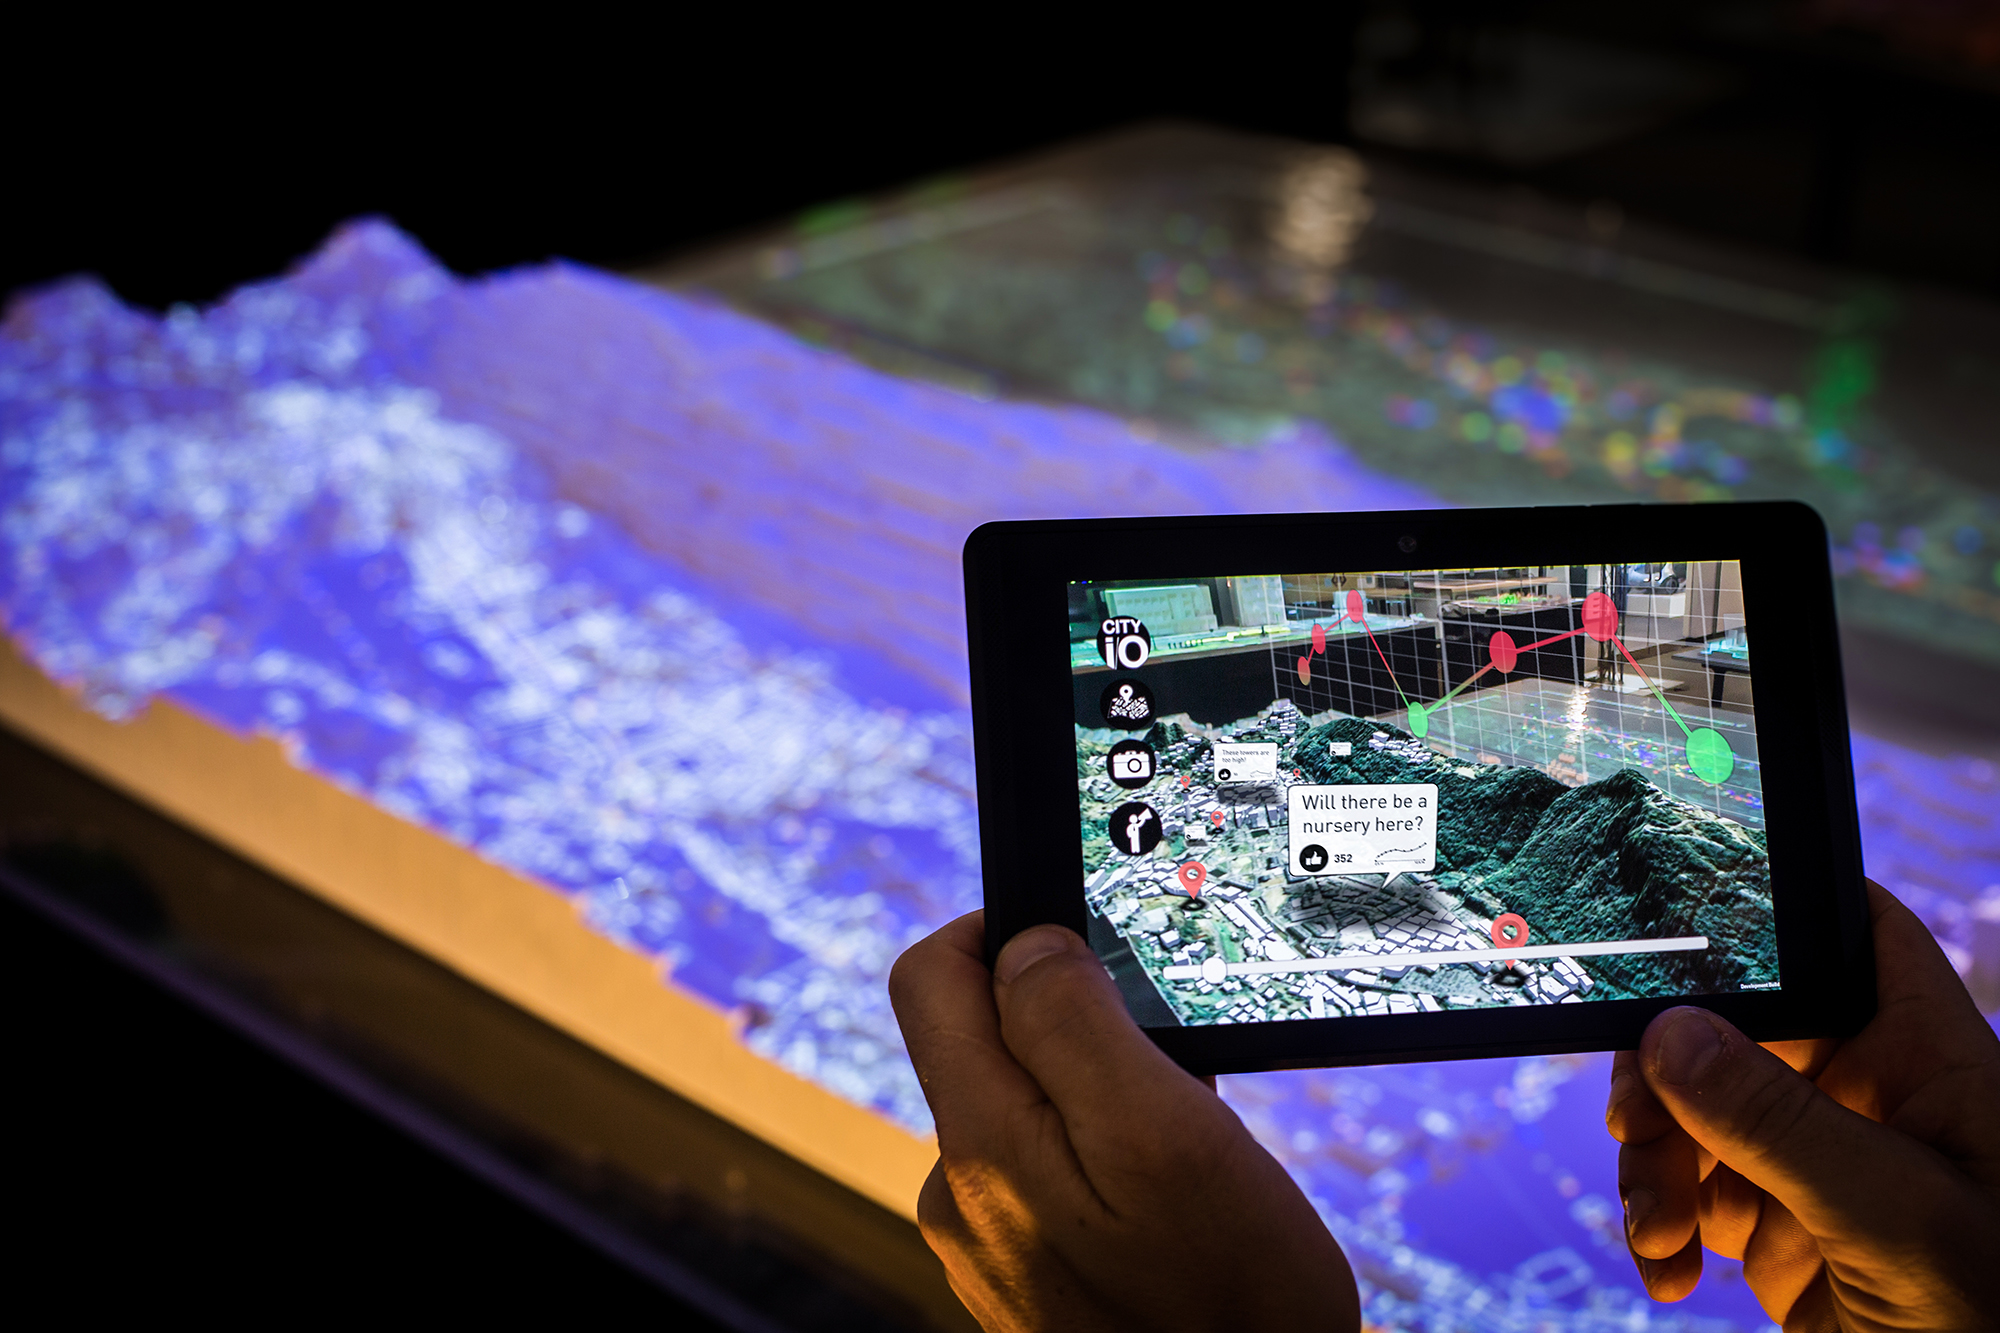
\includegraphics[width=1\textwidth]{chapters/insight/and_abm/figures/and_ar.jpg}
                \end{center}
                \caption{CityScopeAR: Augmented reality platform for CityScope Andorra. Remote participation and complex 3D visualizations are extending the capability of CityScope beyond the limitations of the physical TUI.}
                \label{fig:and_AR}
            \end{figure}

            An Augmented Reality subsystem was designed to allow users to observe spatial, ABM, and interventions data using different devices, client-side applications, web-based interfaces, AR, or VR \cite{noyman2018CityScopeARUD} (for a detailed breakdown of the CityScopeAR system see Section \eqref{sec:cityscope_ar}). The AR subsystem collects data from several sources: (i) Raw telecom data (CDR OD matrix), (ii) Existing built environment, (iii) Real-time 3D representation of design and planning iterations, and (iv) Mobility analysis. In the use-case of Andorra, which is poised in the heart of a sensitive natural landscape, any urban intervention might have major spatial impacts (see Figure \eqref{fig:and_AR}). It is therefore crucial to understand how changes might affect urban form, usability, access, and land-use patterns ahead of urban transformation. The AR layer worked in concert with the TUI, so that users could better sense the spatial implications of urban interventions (see in detail \eqref{ch:transformation} and \eqref{sec:cityscope_ar}).
        }
    }

    \subsection{Discussion}
    {

        \begin{figure}[h]
            \begin{center}
                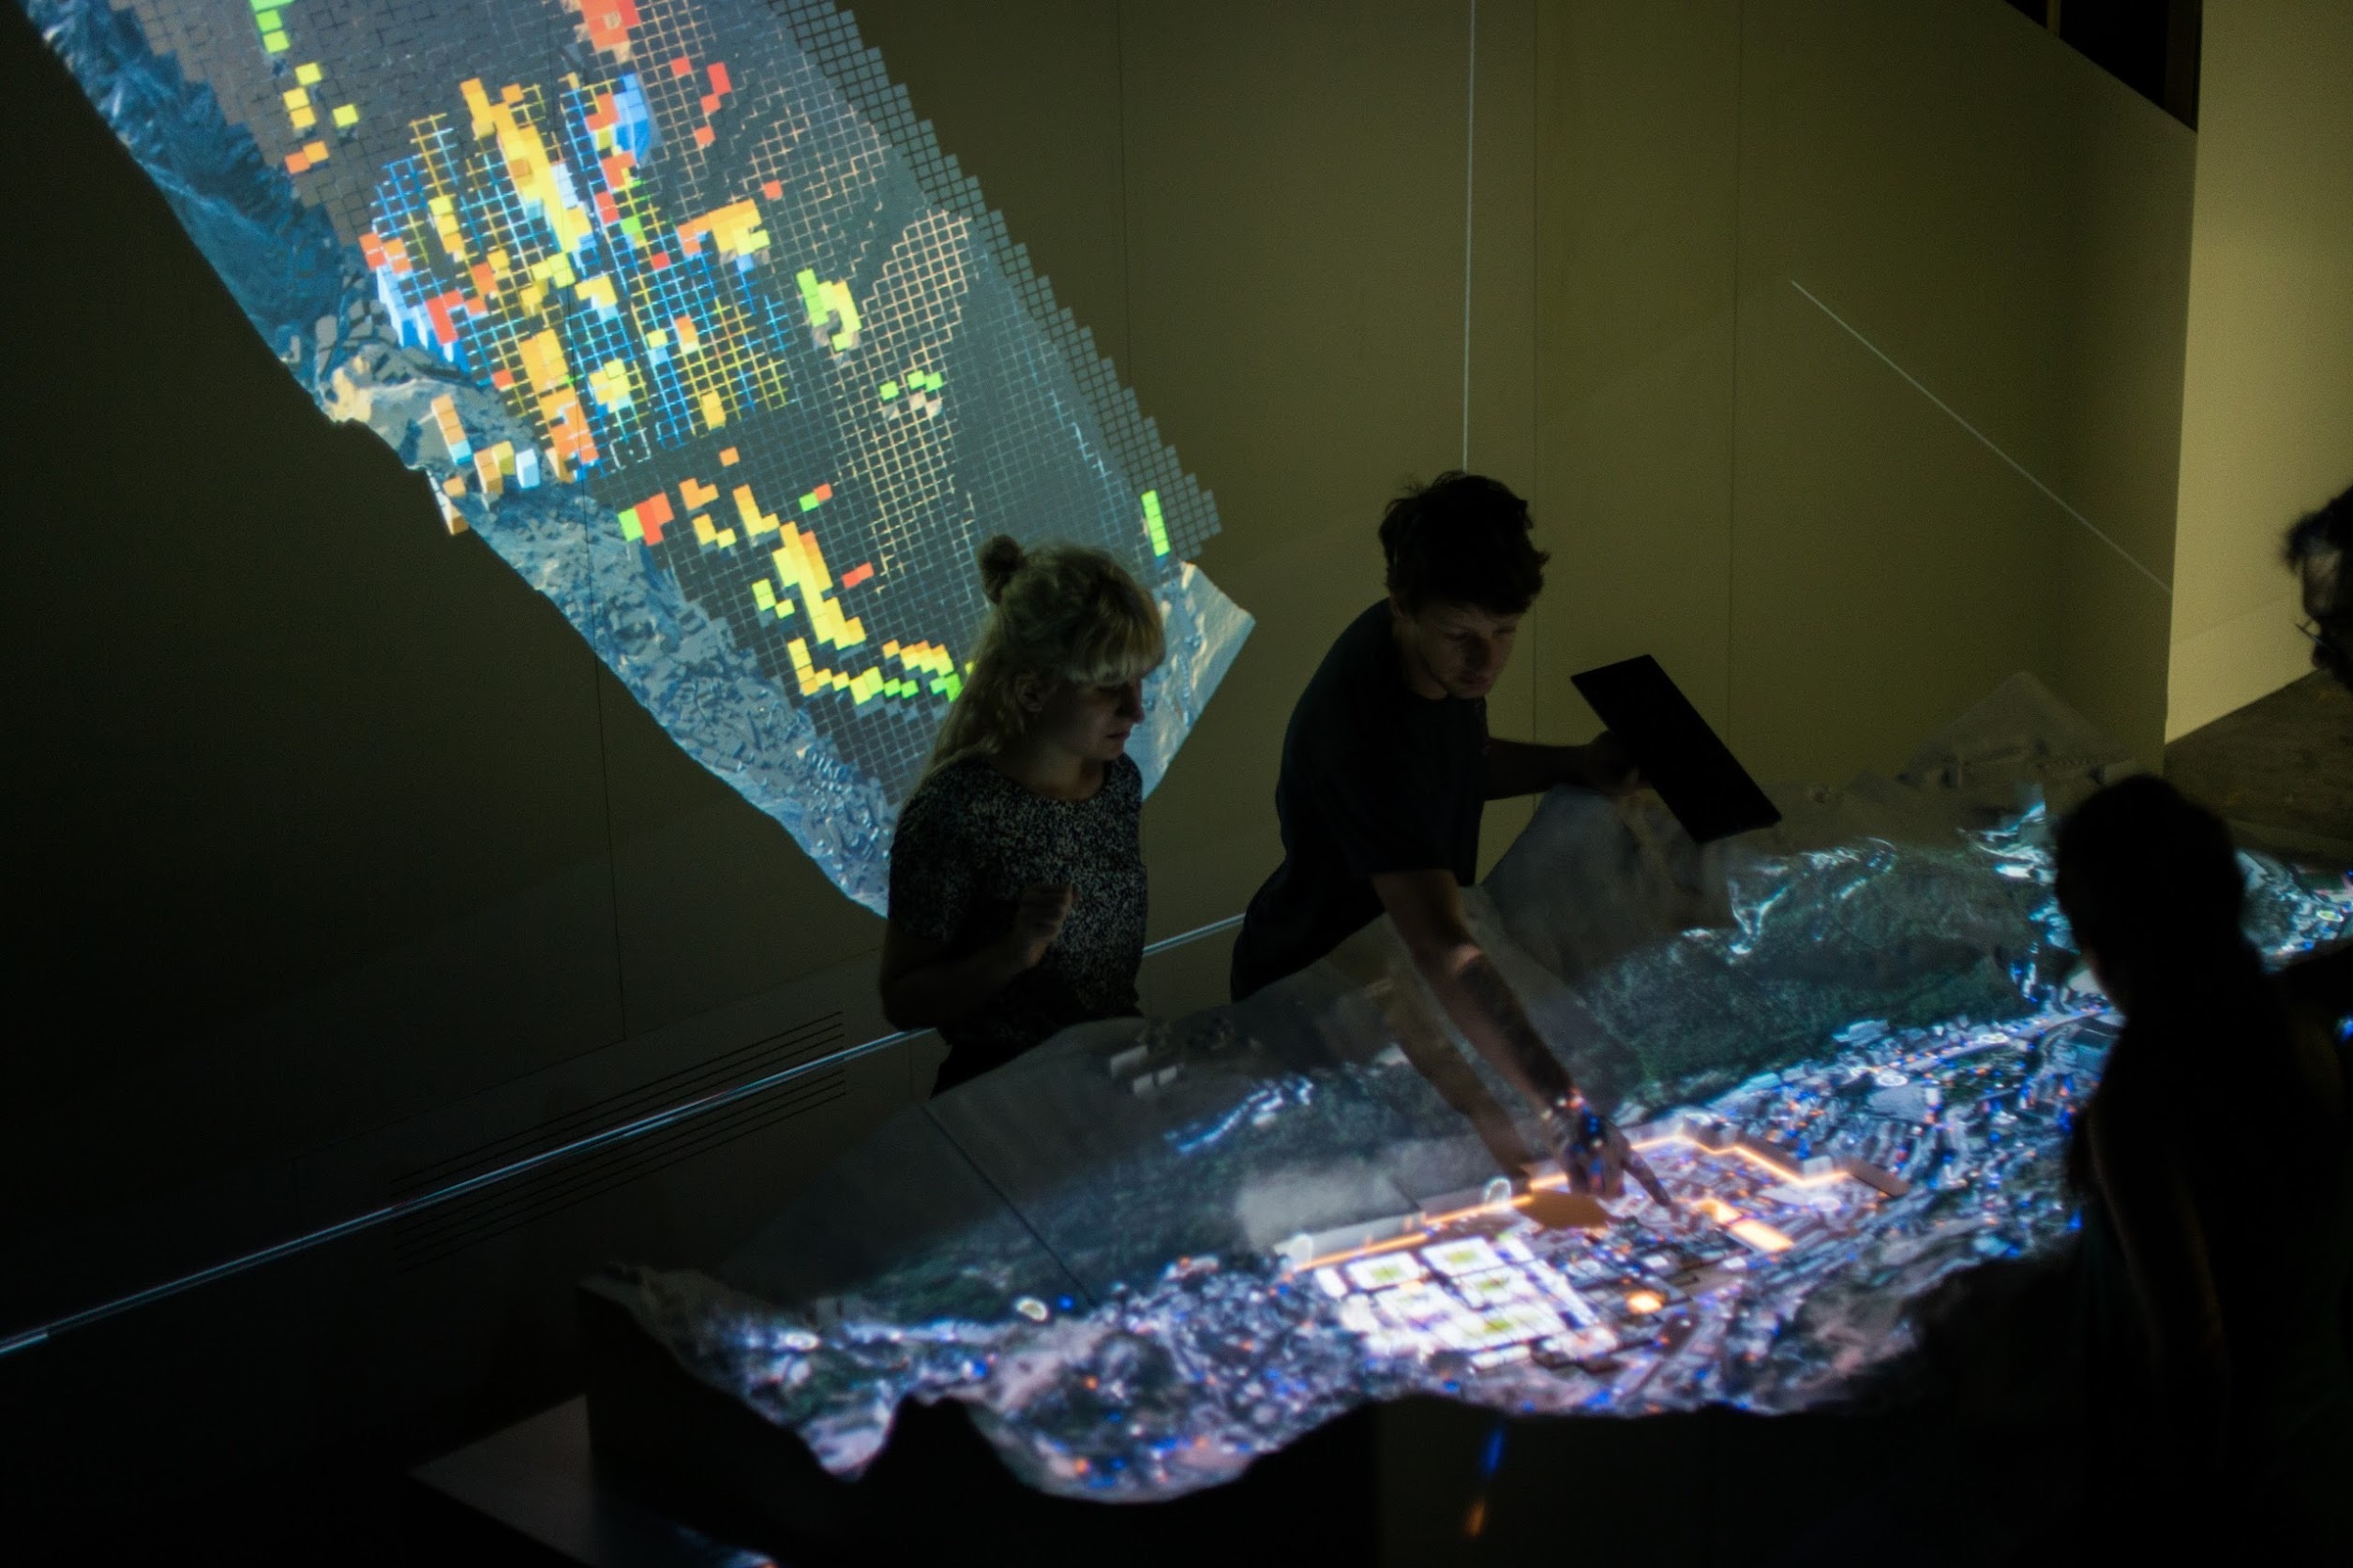
\includegraphics[width=1\textwidth]{chapters/insight/and_abm/figures/and_cs_ppl.jpeg}
            \end{center}
            \caption{CityScope Andorra at the City Science Lab in Caldea, Andorra la Vella. The space is situated in the heart of the city, and was designed to accommodate multi-party discussions, meetings, and events, around a large scale CityScope installation.}
            \label{fig:and_cityscope_ppl}
        \end{figure}


        The Andorra Observatory was developed at MIT (`16-`17), deployed at the Barcelona Smart City Expo World Congress, and was finally mounted in Andorra in late 2017. It was on display in dozens of public demonstrations, and was viewed by thousands of visitors, both at MIT, the City Science Lab in Andorra la-Vella, as well as in the Barcelona Expo in 2016.
        \newline
        The Andorra Observatory was designed to provide a comprehensive view of the city's activity and mobility, and to allow users to interact with the ABM through TUI and AR. The underlining ABM use of CDR data demonstrated the ability to visualize the city's activity and mobility at both local and global levels. As shown in the the rest of this Chapter, the incorporation of better location, spatial, and demographic data can improve the accuracy of such models and the quality of urban insights.

    }
}

